\documentclass[../../../include/open-logic-section]{subfiles}

\begin{document}

\olfileid{sth}{ordinals}{idea}	
\olsection{Gagasan Umum Bab Ordinal}

Pikirna wilangan asli miturut urutan lumrahe:
\begin{center}
	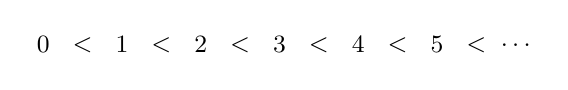
\begin{tikzpicture}
	\foreach \x/\xtext in {0, 1, 2, 3, 4, 5}
	{
		\node (\x a) at (\x, 1) {\small{$\x$}};
		\node (\x a) at (\x.5, 1) {\small{$<$}};
	}
	\node (ldots) at (6, 1) {\small{$\ldots$}};
	\end{tikzpicture}
\end{center}
Ing istilah teknis, iki diarani urutan-$\omega$.
Pancen, urutan umum iki kacermin ing pambangunan wiwitan
tataran-tataran hierarki himpunan. Nanging saiki upamane
kita mindhah $0$ menyang pungkasan urutan iki, supaya
dununge sawisé kabeh wilangan liyane:
\begin{center}
	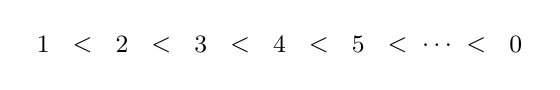
\begin{tikzpicture}
	\foreach \x/\xtext in {1, 2, 3, 4, 5}
	{
		\node (\x a) at (\x, 1) {\small{$\x$}};
		\node (\x a) at (\x.5, 1) {\small{$<$}};
	}
	\node (ldots) at (6, 1) {\small{$\ldots$}};
	\node (bea) at (6.5, 1) {\small{$<$}};
	\node (noa) at (7, 1) {\small{$0$}};
	\end{tikzpicture}
\end{center}
Entitas ing kene tetep padha, nanging urutane beda
kanthi dhasar: urutan kapisan ora nduweni unsur pungkasan,
dene urutan anyar nduweni. Pancen, urutan anyar dumadi
saka urutan-$\omega$ tumrap entitas
($1, 2, 3, 4, 5, \ldots$), banjur disusul entitas liyane.
Iki dadi urutan-$\omega+1$.

Mung nganggo entitas kang padha, kita bisa nggawe luwih
akeh jinis urutan. Contone, pikirna kabeh wilangan genep
(miturut urutan lumrahe), banjur disusul kabeh wilangan
ganjil (miturut urutan lumrahe):
\begin{center}
	\begin{tikzpicture}
	\node(a1) at (1,1) {\small{$0$}};
	\node(a2) at (1.5,1) {\small{$<$}};
	\node(a3) at (2,1) {\small{$2$}};
	\node(a4) at (2.5,1) {\small{$<$}};
	\node(a5) at (3,1) {\small{$4$}};
	\node(a6) at (3.5,1) {\small{$<$}};
	\node(dots) at (4,1) {\small{$\ldots$}};
	\node(aaoe) at (4.5,1) {\small{$<$}};
	\node(b1) at (5,1) {\small{$1$}};
	\node(b2) at (5.5,1) {\small{$<$}};
	\node(b3) at (6,1) {\small{$3$}};
	\node(b4) at (6.5,1) {\small{$<$}};
	\node(b5) at (7,1) {\small{$\ldots$}};
	\end{tikzpicture}
\end{center}
Iki urutan-$\omega$ kang disusul urutan-$\omega$ liyane;
yaiku urutan-$\omega+\omega$.

Kita bisa nerusake maneh. Nanging kang kita karepake
yaiku cara umum kanggo mangerteni maneka \emph{urutan} iki.

\end{document}
